\subsection{Metodi per la gestione dei dati}
In questo sottocapitolo verranno spiegati i metodi studiati ed utilizzati per la gestione dei
dati in python, più nello specifico: come caricare un dataset, una possibile rinomina delle
colonne ralative alle serie per una maggiore comprensione, scelta di un indice, individuazione dei valori
nulli ed infine una sezione relativa al filtraggio.

\paragraph{Cosa viene inteso per dataset} Per dataset si intende un insieme di
serie (nella nostra applicazione temporali) relative ad un'unica applicazione.

\begin{esempio}[\textit{Qualità dell'aria}]
    Consideriamo, per esempio, come applicazione le misurazioni di diversi parametri
    relativi alla qualità dell'aria di Genova: livello di $\mathsf{CO_2}$,
    livello di $\mathsf{SO_2}$, livello di $\mathsf{NO_2}$ e temperatura in \textdegree$\mathsf{C}$.
    In un dataset possiamo considerare ogni parametro come una serie temporale diversa ma indicizzata
    nel tempo in ugual maniera, quindi se queste misurazioni avvengono ogni ora avemo
    per ogni istante di tempo $t$ le misurazioni per ogni parametro in quell'istante.
    \begin{itemize}
        \setlength\itemsep{-0.5em}
        \item $Y_1$: livello di $\mathsf{CO_2}$, $\mathsf{SO_2}$, $\mathsf{NO_2}$ e temperatura in \textdegree$\mathsf{C}$ all'istante $1$.
        \item $Y_2$: livello di $\mathsf{CO_2}$, $\mathsf{SO_2}$, $\mathsf{NO_2}$ e temperatura in \textdegree$\mathsf{C}$ all'istante $2$.
        \item \dots
        \item $Y_T$: livello di $\mathsf{CO_2}$, $\mathsf{SO_2}$, $\mathsf{NO_2}$ e temperatura in \textdegree$\mathsf{C}$ all'istante $T$.
    \end{itemize}
    Ogni parametro in un dataset viene rappresentato come una colonna.
\end{esempio}
Da qusto momento in poi, nel report, quando si parlerà di dataset varrà inteso il tipo
\texttt{pandas.DataFrame}, cioè il modo in cui un dataset viene intrpretato all'interno
di python, mentre per serie si intenderà il tipo \texttt{pandas.Series} oppure un semplice
tipo \texttt{list} di python.

\subsubsection{Pacchetti utilizzati}
Per effettuare tutte le manovre relative all'elaborazione e manipolazione dei dati sono state
utilizzate funzionalità fornite da pacchetti python come \texttt{pandas}, \texttt{numpy} e \texttt{scipy}, essi semplificano
la scrittura di codice e velocizzano il tempo di sviluppo organizzando in maniera ottimale
i dati. Per essere utilizzati essi necessitano prima di essere installati tramite il
gestore di pacchetti di python \texttt{pip}.
\paragraph{Snippet per l'installazione dei pacchetti}
\begin{minted}{bash}
    pip install pandas
    pip install numpy
    pip install scipy
\end{minted}
\paragraph{Snippet per il caricamento in python}
\begin{minted}{python3}
    import pandas as pd
    import numpy as np
    from scipy import signal
\end{minted}



\subsubsection{Caricamento di un dataset}
Per poter utilizzare i dati all'interno di python è stata utilizzata
la funzionalità di pandas \texttt{read\_csv} dove, ogni colonna fa riferimento 
ad una serie.
\paragraph{Snippet}
\begin{minted}{python3}
    dataset = pd.read_csv('data.csv')
\end{minted}





\subsubsection{Rinomina delle colonne relative alle serie}
In qualche case, il primo passo da eseguire, è quello di rinominare
le colonne relative ad ogni serie così da poter avere una rappresentazione
più accurata del dataset.
Tramite l'utilizzo della funzione \texttt{display} e del metodo \texttt{head}
del dataset possiamo controllare i primi $5$ valori di un dataset
controllando anche così il nome di ogni colonna.
\paragraph{Snippet}
\begin{minted}{python3}
    display(dataset.head())
\end{minted}
\begin{figure}[h!]
    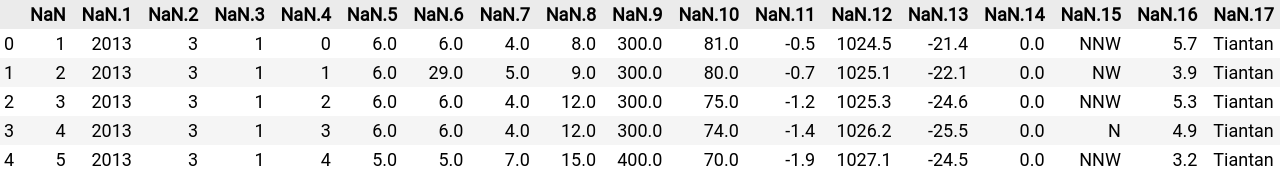
\includegraphics[width=\linewidth,height=2.7cm]{head_before_rename.png}
    \caption{output del metodo head prima della rinomina delle colonne}
    \label{fig:head_before_rename}
\end{figure}
Come si può notare nell'immagine~\ref*{fig:head_before_rename} i nomi delle colonne 
non hanno nessun nome significativo, con il seguente esempio potremmo
cambiare il nome delle colonne.

\paragraph{Snippet}
\begin{minted}{python3}
    # definizione di una lista di nomi per le colonne del dataset
    dataset.columns = [ 'no',    'year',  'month', 'day', 'hour', 
                        'pm2_5', 'pm10',  'so2',   'no2', 'co',  
                        'o3',    'temp',  'pres',  'dewp','rain',  
                        'wd',    'wspm',  'station']
    display(dataset.head())
\end{minted}
\begin{figure}[h!]
    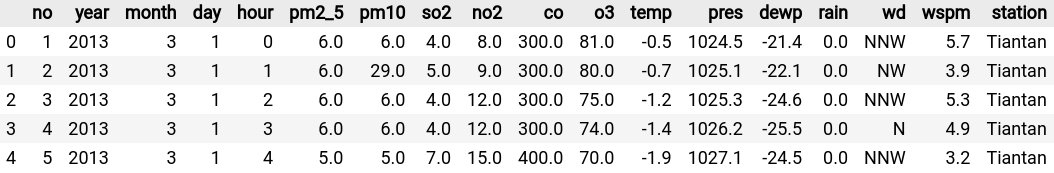
\includegraphics[width=\linewidth,height=2.7cm]{head_after_rename.png}
    \caption{output del metodo head dopo la rinomina delle colonne}
    \label{fig:head_after_rename}
\end{figure}
Come si può notare nell'immagine~\ref*{fig:head_after_rename}
assegnando la lista delle colonne come attuali nomi per le serie del dataset
riusciamo ad ottenere un'interpretazione più accurata.


\subsubsection{Scelta dell'indice}
Molte delle funzionalità fornite da \texttt{pandas} ed altri pacchetti python
richiedono che il dataset sia indicizzato nel tempo nel corretto modo.
In figura~\ref*{fig:head_after_rename} si può notare che la prima colonna
senza nome e la seconda colonna con nome \texttt{no}, indichino
il numero di riga per ogni misurazione, la differenza è che la prima colonna
è generata automaticamente dal pacchetto \texttt{pandas}, ed impostata
di default come indice, mentre la seconda con
nome \texttt{no} è fornita direttamente dal file csv precedentemente caricato.
Per l'analisi della maggior parte delle serie temporali un'idicizzazione per numero
di riga non è significativa, sarebbe molto più conveniente lavorare avendo
come indice di tabella la data ed ora di ogni effettiva misurazione.
A questo proposito il dataset caricato ci fornisce delle colonne (\texttt{year}
, \texttt{month}, \texttt{day} e \texttt{hour}) indicizzate per tempo e relative
ad ogni misurazione, che possono essere riformattate insieme ed usate come indice
per il dataset.

\paragraph{Snippet}
\begin{minted}{python3}
    # unificazione delle colonne relative al tempo per ogni 
    # istante di tempo t in una nuova colonna
    new_index_column = []
    for i in range(len(dataset.year)):
    new_index_column.append("%s/%s/%s %s:0:0" 
        % (dataset.day[i], dataset.month[i], 
           dataset.year[i], dataset.hour[i]) )

    # elimina le colonne relative al tempo
    del dataset["year"], dataset["month"], 
        dataset["day"], dataset["hour"], 
        dataset["no"]

    # imposta/crea la nuova colonna date e converti in datetime
    dataset['date'] = new_index_column
    dataset['date'] = pd.to_datetime(dataset.date, dayfirst=True)

    # imposta come index la nuova colonna date
    dataset.set_index("date", inplace=True)
    display(dataset.head())
\end{minted}
\begin{figure}[h!]
    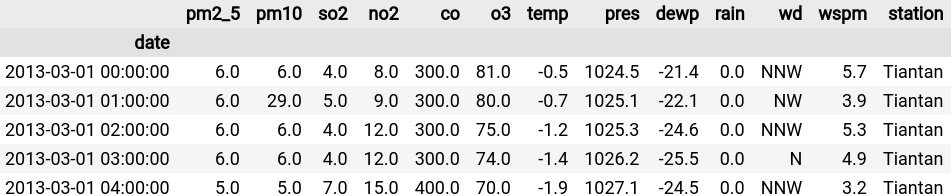
\includegraphics[width=\linewidth,height=2.7cm]{head_after_index_set.png}
    \caption{output del metodo head dopo aver impostato l'indice}
    \label{fig:head_after_index_set}
\end{figure}
Come si può notare dall'output del metodo \texttt{head} nell'immagine \ref*{fig:head_after_index_set}
\texttt{date} è stato impostato come indice di tabella e quindi da questo momento in poi
possiamo accedere al dataset, scegliendo le misurazioni interessate, utilizzando la
data.

\paragraph{Periodo di campionamento}
Un'altra importante modifica è impostare il periodo di campionamento del dataset,
in poche parole impostare un corretto indice non basta a massimizzare il corretto
funzionamento delle funzionalità di analisi delle serie temporali, bisogna anche specificare
l'istante di tempo che occorre tra una misurazione e l'altra. Per fare ciò
\texttt{pandas} fornise un metodo che imposta il periodo di campionamento
a quello deiderato, nel nostro caso sappiamo che le misurazioni sono state campionate
ogni ora.
\subparagraph{Snippet}
\begin{minted}{python3}
    # imposta il periodo di capionamento 
    # del dataset ad ogni ora
    dataset = dataset.asfreq("h")
\end{minted}

\subsubsection{Individuazione dei valori nulli e possibili soluzioni}
La presenza di valori nulli in una serie può avere molteplici cause, ad esempio,
l'impossibilità da parte dello strumento di capionare ad un certo istante di tempo $t$,
oppure se pensiamo ad una fotocamera che acquisisce delle coordinate relative ad un soggeto,
l'usicta di esso dall'obbiettivo.

Indifferentemente dal motivo per cui dei valori nulli sono presenti, 
in una serie o un dataset, la loro presenza può causare molti
problemi sia nel corretto funzionamento di alcune funzionalità per l'analisi sia perchè
non avere dei valori in determinati punti della serie, in certe applicazioni, potrebbe
essere un problema. \texttt{pandas} fornisce dei metodi utili, e semplici, alla soluzione di questo
problema ma ovviamente ogni problema è diverso e quindi, per applicazioni specifiche,
potrebbe essere necessario cercare soluzioni differenti. In questa sezione ci limitiamo
a descrivere le funzionalità fornite da \texttt{pandas} per la soluzione a questo problema.

\paragraph{Controllo}
Per controllare la presenza di valori nulli \texttt{pandas} fornisce un metodo chiamato
\texttt{isna} che ritorna un dataset dove, per ogni misurazione, indica \texttt{True}
se la misurazione è \texttt{NaN} altrimenti \texttt{False}. Sommando i valori \texttt{True}
per ogni colonna possiamo controllare quanti valori nulli sono presenti per ogni serie.\\
\\
\subparagraph*{Snippet}
\begin{minted}{python3}
    # controllo valori nulli
    dataset.isna().sum()
\end{minted}
\begin{figure}[h!]
    \centering
    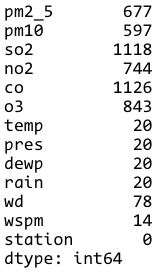
\includegraphics[width=0.24\linewidth,height=5cm]{somma_valori_nulli.png}
    \caption{output della somma dei valori nulli relativi ad ogni serie del dataset}
    \label{fig:sum_null}
\end{figure}
Come si puo notare dall'output del comando in figura~\ref*{fig:sum_null}
il nostro dataset contiene molteplici valori nulli, ora vediamo come poter risolvere
il segente problema

\paragraph{Back fill o Forward fill}
\texttt{pandas} fornisce la possibilità di ``riempire'' i valori nulli in due diverse
modalità tramite l'utilizzo del metodo \texttt{fillna}
\begin{itemize}
    \item \textbf{Back fill}: permette di sostituire i valori nulli con la succesiva
    misurazione valida.
    \item \textbf{Forward fill}:  permette di sostituire i valori nulli propagando
    l'ultima valida misurazione alla prossima valida.
\end{itemize}
Entrambi i metodi gestiscono i valori nulli più o meno nella stessa maniera ma la scelta
di uno piuttosto che l'altro cambia da caso in caso dipendendtemente dal risultato
ottenuto dopo l'utilizzo di essi.


Per i nostri esempi il risulato nell'utilizzo di un metodo piuttosto che l'altro
portava comunque ad un risultato soddisfacente.\\
\\
\subparagraph*{Snippet}
\begin{minted}{python3}
    # rimepimento dei valori nulli 
    # mediante il metodo di forward fill
    dataset = dataset.fillna(method="ffill")
    dataset.isna().sum()
\end{minted}
\begin{figure}[h!]
    \centering
    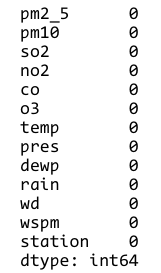
\includegraphics[width=0.24\linewidth,height=5cm]{somma_valori_nulli_dopo_fill.png}
    \caption{output della somma dei valori nulli relativi ad ogni serie del dataset dopo l'utilizzo del metodo \texttt{fillna}.}
\end{figure}


\paragraph{Interpolazione} 
Un possibile metodo, non fornito dalle funzionalità del pacchetto \texttt{pandas},
che potrebbe essere utilizzato è quello di interpolare i dati così da poter colmare
i vuoti creati dai valori nulli. Questa funzionalità non è stata sviluppata
in quanto non fine allo scopo di questo tirocinio ma, in certe applicazioni, si potrebbe
voler utilizzare una metodologia basata su questa tecnica per ottenere una rappresentazione
più accurata dei dati.


\paragraph{Altro metodo non convenzionale}
Un altro metodo non convenzionale, non presente tra le funzionalità fornite,
è quello di poter eliminare i valori nulli dalle serie semplicemente
eliminandoli. Ovviamente questo concetto di eliminare una misurazione nulla va
contro a tutte le premesse fatte fino ad ora, non avendo così una ``reale''
serie temporale poichè mancherebbe una misurazione ad un determinato istante di tempo
$t$, e molte delle analisi che si vorrebbero poter fare su una serie risulterebbero
inapplicabili. 
Tuttavia, in qualche applicazione particolare (come vedremo in seguito), una funzionalità
che semplicemente elimina i valori nulli da una serie potrebbe tornare comoda.
\subparagraph*{Snippet}
\begin{minted}{python3}
    import math as math # import del pacchetto math

    def delete_nan(series: pd.Series | list):
    """ emlimina i valori nulla da una serie
    """
    new_series = []
    for idx, value in enumerate(series):
        if not math.isnan(value):
            new_series.append(value)
    return np.array(new_series)
\end{minted}


\subsubsection{Filtraggio}
Nella maggior parte dei casi quando si parla di serie temporali fonite direttamente 
da apparecchiature che eseguono le misurazioni, i dati si presentano in maniera
``grezza'' ed è quindi necessario filtrarli per poter rimuovere una buona parte
del rumore presente. Questo passaggio è molto importante se parliamo di dati non elaborati
in quanto avere del rumore in una serie temporale o, più in generale, in qualsiasi
tipo di segnale, porta a leggere delle misurazioni ``false''. Solitamente il rumore
indesiderato risiede nelle frequenze alte del segnale, quindi, a questo proposito,
vediamo come poter filtrare una sorgente ``grezza'' di dati mediante l'utilizzo del
modulo \texttt{signal} del pacchetto \texttt{scipy}.
